\documentclass[a4paper, 11pt, amsmath, graphicx]{article}\usepackage[]{graphicx}\usepackage[]{color}
%% maxwidth is the original width if it is less than linewidth
%% otherwise use linewidth (to make sure the graphics do not exceed the margin)
\makeatletter
\def\maxwidth{ %
  \ifdim\Gin@nat@width>\linewidth
    \linewidth
  \else
    \Gin@nat@width
  \fi
}
\makeatother

\definecolor{fgcolor}{rgb}{0.345, 0.345, 0.345}
\newcommand{\hlnum}[1]{\textcolor[rgb]{0.686,0.059,0.569}{#1}}%
\newcommand{\hlstr}[1]{\textcolor[rgb]{0.192,0.494,0.8}{#1}}%
\newcommand{\hlcom}[1]{\textcolor[rgb]{0.678,0.584,0.686}{\textit{#1}}}%
\newcommand{\hlopt}[1]{\textcolor[rgb]{0,0,0}{#1}}%
\newcommand{\hlstd}[1]{\textcolor[rgb]{0.345,0.345,0.345}{#1}}%
\newcommand{\hlkwa}[1]{\textcolor[rgb]{0.161,0.373,0.58}{\textbf{#1}}}%
\newcommand{\hlkwb}[1]{\textcolor[rgb]{0.69,0.353,0.396}{#1}}%
\newcommand{\hlkwc}[1]{\textcolor[rgb]{0.333,0.667,0.333}{#1}}%
\newcommand{\hlkwd}[1]{\textcolor[rgb]{0.737,0.353,0.396}{\textbf{#1}}}%

\usepackage{framed}
\makeatletter
\newenvironment{kframe}{%
 \def\at@end@of@kframe{}%
 \ifinner\ifhmode%
  \def\at@end@of@kframe{\end{minipage}}%
  \begin{minipage}{\columnwidth}%
 \fi\fi%
 \def\FrameCommand##1{\hskip\@totalleftmargin \hskip-\fboxsep
 \colorbox{shadecolor}{##1}\hskip-\fboxsep
     % There is no \\@totalrightmargin, so:
     \hskip-\linewidth \hskip-\@totalleftmargin \hskip\columnwidth}%
 \MakeFramed {\advance\hsize-\width
   \@totalleftmargin\z@ \linewidth\hsize
   \@setminipage}}%
 {\par\unskip\endMakeFramed%
 \at@end@of@kframe}
\makeatother

\definecolor{shadecolor}{rgb}{.97, .97, .97}
\definecolor{messagecolor}{rgb}{0, 0, 0}
\definecolor{warningcolor}{rgb}{1, 0, 1}
\definecolor{errorcolor}{rgb}{1, 0, 0}
\newenvironment{knitrout}{}{} % an empty environment to be redefined in TeX

\usepackage{alltt}
% R vignette preable

\usepackage{amsmath}
\usepackage{mathtools}
\usepackage{amsfonts}
\usepackage{amssymb}
\usepackage{hyperref}

\usepackage{geometry}
 \geometry{
 a4paper,
 total={170mm,257mm},
 left=20mm,
 top=20mm,
 }
 
\usepackage{fancyhdr}
\pagestyle{fancy}
\renewcommand{\headrulewidth}{0pt}
\renewcommand{\footrulewidth}{0pt}
\setlength\headheight{80.0pt}
\addtolength{\textheight}{-80.0pt}
\lhead{
\includegraphics[width=0.34\textwidth]{UoLLogoMono.pdf}}

\def\bmu{{\mbox{\boldmath $\mu$}}}
\def\bt{{\mbox{\boldmath $\theta$}}}
\def\bs{{\mbox{\boldmath $\sigma$}}}
\IfFileExists{upquote.sty}{\usepackage{upquote}}{}
\begin{document}
\title{3. Gaussian relationships}
\author{Simon Vaughan \thanks{Email: sav2@le.ac.uk}}
\maketitle

In this section we discuss some of the connections between Gaussian distributions in differing dimensions.

%%%%%%%%%%%%%%%%%%%%%%%%%%%%%%%%%%%%%%%%%%%%%%%
\vspace{0.4cm}
\textbf{The bivariate (two dimensional) Gaussian}
\\

The bivariate Gaussian pdf is given by 

\begin{equation}
\label{eqn:bi}
  p(\mathbf{y}|\bmu, \Sigma) = \frac{1}{ (2 \pi)^{M/2} |\Sigma|^{1/2} } 
                 \exp \left( -\frac{1}{2} (\mathbf{y} - \bmu)^T
                 \Sigma^{-1} (\mathbf{y} - \bmu) \right)
\end{equation}

where $\mathbf{y} = (y_1, y_2)^T$, $\bmu = (\mu_1, \mu_2)^T$ are the $2$-vector means of each variables and $\Sigma$ is the $2 \times 2$ symmetric covariance matrix

\begin{equation}
  \Sigma = \left[ \begin{matrix}
 a & c \\
 c & b 
 \end{matrix} \right]
\end{equation}

The diagonal elements ($a$ and $b$) are the variances of $y_1$ and $y_2$, respectively, e.g. $var(y_1) = \sigma_{y1}^2 = a$. The off-diagonal element $c$ is the covariance of $y_1$ and $y_2$.

%%%%%%%%%%%%%%%%%%%%%%%%%%%%%%%%%%%%%%%%%%%%%%%
\vspace{0.4cm}
\textbf{Marginal and conditional densities}
\\

Writing $p(\mathbf{y}) = p(y_1, y_2)$ we see that this is the \emph{joint} distribution of $y_1$ and $y_2$. We can use the rules of probability theory (see e.g. chapter 4 of \emph{Scientific Inference}) to rewrite this as

\begin{equation}
\label{eqn:marg0}
  p(y_1, y_2) = p(y_1 | y_2) p(y_2) = p(y_2 | y_1) p(y_1)
\end{equation}

Here $p(y_1|y_2)$ is a \emph{conditional distribution} for $y_1$ given $y_2$. It is a density for $y_1$, once we are given a value for $y_2$. And $p(y_2)$ is a \emph{marginal} distribution for $y_2$. It is a density for $y_2$ irrespective of $y_1$. 

A \emph{marginal} distribution is obtained by `integrating out' some of the variables. In the bivariate case we have two possible marginal distributions

\begin{align}
\label{eqn:cond1}
p(y_1) & = \int_{-\infty}^{+\infty} p(y_1, y_2) dy_2 \\
       & = \int_{-\infty}^{+\infty} p(y_1 | y_2) p(y_2) dy_2
\end{align}

and also
\begin{align}
\label{eqn:cond2}
p(y_2) & = \int_{-\infty}^{+\infty} p(y_1, y_2) dy_1\\
       & = \int_{-\infty}^{+\infty} p(y_2 | y_1) p(y_1) dy_1
\end{align}

We can think of the marginal distribution $p(y_1)$ as the probability density of $y_1$ irrespective of $y_2$. We take the conditional density, which tells us how $y_1$ is distributed given a value for $y_2$, and we average this over the distribution of $y_2$.

%%%%%%%%%%%%%%%%%%%%%%%%%%%%%%%%%%%%%%%%%%%%%%%
\vspace{0.4cm}
\textbf{Gaussian marginal distributions}
\\

The marginal distribution of a multivariate Gaussian is another Gaussian. So its density has the same form as equation \ref{eqn:bi}, but the mean $\bmu$ and covariance matrix $\Sigma$ are replaced by the vector and matrix formed from subsets of the mean vector and covariance matrix of the joint density.

In the bivariate case, the marginal density for $y_1$ is obtained by taking $\bmu = \mu_1$ and $\Sigma = a$. We get

\begin{align}
  p(y_1|\bmu,\Sigma) & = \frac{1}{ (2 \pi) |a|^{1/2} } 
                 \exp \left( - \frac{1}{2} (y_1 - \mu_1)
                 a^{-1} (y_1 - \mu) \right) \\
         & = \frac{1}{ 2 \pi \sigma_{y1}^2 } 
                 \exp \left( - \frac{1}{2} \frac{(y_1 - \mu_1)^2}{\sigma_{y1}^2}
                 \right)
\end{align}

and we would get a similar expression for $p(y_2)$. This is just another Gaussian distribution.

\begin{figure}
  \centering
  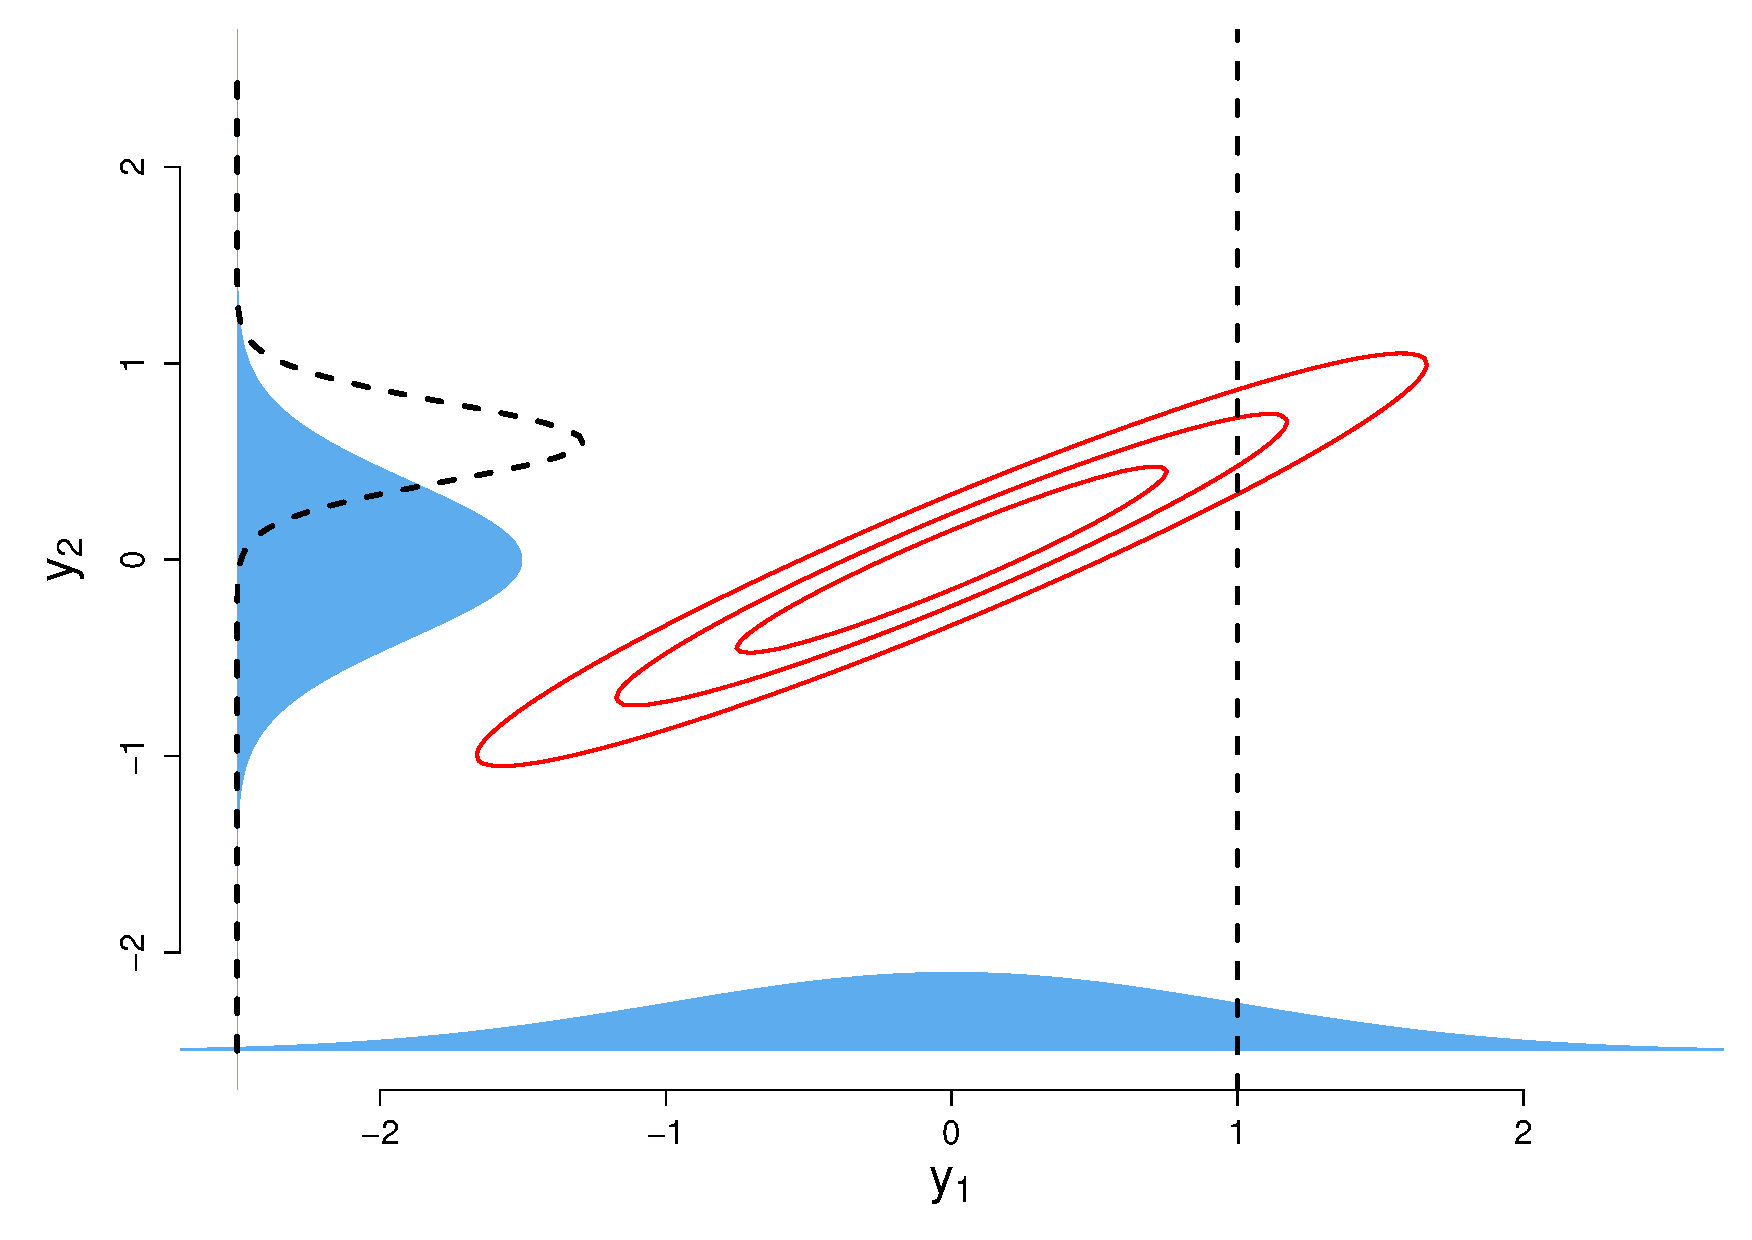
\includegraphics[width = 4in]{Gaussian2d.pdf}
  \caption{The contours represent a bivariate Gaussian density $p(y_1, y_2$). The solid blue curves on the bottom and left are the marginal densities $p(y_1)$ and $p(y_2)$, respectively. The dashed curve is the conditional density $p(y_2|y_1=1)$, with the line $y_1 = 1$ also marked as a dashed line.}
\end{figure}

Similar rules apply for higher dimentional Gaussian distributions. If we partition an $n$-dimensional vector $\mathbf{y}$ into

\begin{equation}
\mathbf{y} = \left[ \begin{matrix} \mathbf{y}_1 \\ \mathbf{y}_2 \end{matrix} \right]
\end{equation}

where $\mathbf{y}_1$ is an $l$-dimensional vector and $\mathbf{y}_2$ is an $m$-dimensional vector ($n = l + m$). We can partition the mean vector and covariance matrix in a similar manner

\begin{equation}
\bmu = \left[ \begin{matrix} \bmu_1 \\ \bmu_2 \end{matrix} \right]
\end{equation}

and

\begin{equation}
  \Sigma = \left[ \begin{matrix}
  A & C^T \\
  C & B
  \end{matrix} \right]
\end{equation}

where $A$, $B$, $C$ are matrices (sizes $l \times l$, $m \times m$ and $m \times l$, respectively). 

The (marginal) density $p(\mathbf{y}_1)$ of the $l$-dimensional vector $\mathbf{y}_1$ is a Gaussian with mean vector $\bmu_1$ and covariance matrix $A$.

%%%%%%%%%%%%%%%%%%%%%%%%%%%%%%%%%%%%%%%%%%%%%%%
\vspace{0.4cm}
\textbf{Gaussian conditional distributions}
\\

Similarly, if we have a bivariate Gaussian density $p(y_1, y_2)$, the conditional distribution of $y_1$ given $y_2$ is also a Gaussian. 

\begin{equation}
  p(y_2|y_1) = \frac{ p(y_1, y_2) }{ p(y_1) }
\end{equation}

(compare with eqn \ref{eqn:cond2}). After some messy algebra (!) it is possible to show that -- with $y_1$ constant -- this has a Gaussian distribution with mean and variance

\begin{align}
  \mu_{2|1} & = \mu_2 + c(y_1 - \mu_1) / a   \\
  \sigma_{2|1}^2 & = b - c a^{-1} c
\end{align}

Similarly, the conditional distribution of vector $\mathbf{y}_2$ given $\mathbf{y}_1$ is also a Gaussian. In this case the mean and covariance are given by 

\begin{equation}
  mean(\mathbf{y}_2|\mathbf{y}_1) = \bmu_2 + C A^{-1} (\mathbf{y}_1 - \bmu_1)
\end{equation}

and

\begin{equation}
  cov(\mathbf{y}_2|\mathbf{y}_1) = B - CA^{-1} C^T
\end{equation}

(A proof of this can be found in many good books on multivariate statistics.) If we know (or assume) the mean of $\mathbf{y}$ is a constant scalar ($\bmu = \mu$) then we can write $\mathbf{y}_1' = \mathbf{y}_1 - \mu$.

\begin{equation}
  \mathbf{y}_2|\mathbf{y}_1 \sim N(\overline{\mathbf{y}_2}, D)
\end{equation}

i.e. $\mathbf{y}_2$ given $\mathbf{y}_1$ is distributed as a Gaussian with mean 

\begin{equation}
\label{eqn:condmean}
  \overline{\mathbf{y}_2} = \mu + C A^{-1} \mathbf{y}_1' 
\end{equation}

and covariance matrix 

\begin{equation}
\label{eqn:condcov}
  D = B - CA^{-1} C^T
\end{equation}

The matrix $D$ is known as the `Schur complement of $A$ in $\Sigma$' (sometimes written $\Sigma / A$).

Equation \ref{eqn:condmean} might seem odd. Didn't we already assume the mean value was $\bmu=\mu$? Yes, but that is an average over all realisations of the process. Once we have observed some value for $y$ at time $t$ we can make a more informed prediction of the value $y_*$ at some nearby time $t_*$ based on our knowledge of the covariance function. If the covariance function produces slowing varying curves then our estimate of $y_*$ should be close to $y$. We use our knowledge of the covariance function and the data to improve estimates of any other $y_*$, for this particular realisation of the process. 

Also, equation \ref{eqn:condcov} seems odd, in the sense that it makes no use of the known values $\mathbf{y}_1$. The output covariance $D$ depends only on the input times of the known values ($\mathbf{t_1}$), the times at which we wish to prediction ($\mathbf{t}_2$), and the auto-covariance function. Equation \ref{eqn:condcov} gives the covariance for $\mathbf{y}_2$ as the difference between two terms. The first is simply the covariance of $\mathbf{y}_2$ in the absence of any information about $\mathbf{y}_1$ (the marginal distribution of $\mathbf{y}_2$). The second term is positive, and makes use of information about the times of the known vaues ($\mathbf{t}_1$) and the autocovariance function to `bring down the error' on $\mathbf{y}_2$ near times where the values of $\mathbf{y}_1$ provide information.

%%%%%%%%%%%%%%%%%%%%%%%%%%%%%%%%%%%%%%%%%%%%%%%
\vspace{0.4cm}
\textbf{Worked example}
\\

Let's simulate a GP at $m=500$ times.

\begin{knitrout}
\definecolor{shadecolor}{rgb}{0.969, 0.969, 0.969}\color{fgcolor}\begin{kframe}
\begin{alltt}
\hlcom{# define vector of times for observations}
\hlstd{m} \hlkwb{<-} \hlnum{500}
\hlstd{t.f} \hlkwb{<-} \hlkwd{seq}\hlstd{(}\hlopt{-}\hlnum{0.5}\hlstd{,} \hlnum{1.5}\hlstd{,} \hlkwc{length} \hlstd{= m)}
\end{alltt}
\end{kframe}
\end{knitrout}

Now, we must define the ACV 

\begin{knitrout}
\definecolor{shadecolor}{rgb}{0.969, 0.969, 0.969}\color{fgcolor}\begin{kframe}
\begin{alltt}
\hlcom{# define covariance function}
\hlstd{acv} \hlkwb{<-} \hlkwa{function}\hlstd{(}\hlkwc{tau}\hlstd{,} \hlkwc{theta}\hlstd{) \{}
  \hlstd{A} \hlkwb{<-} \hlkwd{abs}\hlstd{( theta[}\hlnum{1}\hlstd{] )}
  \hlstd{l} \hlkwb{<-} \hlkwd{abs}\hlstd{( theta[}\hlnum{2}\hlstd{] )}
  \hlstd{acov} \hlkwb{<-} \hlstd{A} \hlopt{*} \hlkwd{exp}\hlstd{(}\hlopt{-}\hlnum{0.5} \hlopt{*} \hlstd{(tau} \hlopt{/} \hlstd{l)}\hlopt{^}\hlnum{2}\hlstd{)}
  \hlkwd{return}\hlstd{(acov)}
\hlstd{\}}
\end{alltt}
\end{kframe}
\end{knitrout}

Notice how this takes two inputs: {\tt tau} is a matrix of all the $\tau_{ij} = |t_i - t_j|$ values, and {\tt theta} is a vector listing the parameters needed to specify the ACV, i.e. $\bt = \{ A, l \}$. For `safety' reasons we use the absolute value of these to ensure that they do not become negative, which could produce an invalid ACV.

Then we define the mean $\bmu = 0$ and  populate the elements of the desired covariance matrix $S$

\begin{knitrout}
\definecolor{shadecolor}{rgb}{0.969, 0.969, 0.969}\color{fgcolor}\begin{kframe}
\begin{alltt}
\hlstd{mu} \hlkwb{<-} \hlkwd{array}\hlstd{(}\hlnum{0}\hlstd{,} \hlkwc{dim} \hlstd{= m)}        \hlcom{# set all means to zero}
\hlstd{tau} \hlkwb{<-} \hlkwd{abs}\hlstd{(} \hlkwd{outer}\hlstd{(t.f, t.f,} \hlstr{"-"}\hlstd{) )} \hlcom{# compute t_j - t_i}
\hlstd{theta} \hlkwb{<-} \hlkwd{c}\hlstd{(}\hlnum{1.0}\hlstd{,} \hlnum{0.1}\hlstd{)}           \hlcom{# define ACV parameters}
\hlstd{S} \hlkwb{<-} \hlkwd{acv}\hlstd{(tau, theta)}           \hlcom{# acf(tau) gives S_\{ij\} matrix}
\hlkwd{diag}\hlstd{(S)} \hlkwb{<-} \hlkwd{diag}\hlstd{(S)} \hlopt{+} \hlnum{1e-5}      \hlcom{# add a tiny 'epsilon' to help ensure pos. def.}
\end{alltt}
\end{kframe}
\end{knitrout}

Now we can use what we know about simulating GPs to produce a realisation.

\begin{knitrout}
\definecolor{shadecolor}{rgb}{0.969, 0.969, 0.969}\color{fgcolor}\begin{kframe}
\begin{alltt}
\hlcom{# produce Gaussian vector}
\hlstd{f} \hlkwb{<-} \hlstd{mvtnorm}\hlopt{::}\hlkwd{rmvnorm}\hlstd{(}\hlnum{1}\hlstd{,} \hlkwc{mean} \hlstd{= mu,} \hlkwc{sigma} \hlstd{= S,} \hlkwc{method} \hlstd{=} \hlstr{"chol"}\hlstd{)}

\hlcom{# plot the 'true' function f(t)}
\hlkwd{plot}\hlstd{(t.f, f,} \hlkwc{type} \hlstd{=} \hlstr{"l"}\hlstd{,} \hlkwc{bty} \hlstd{=} \hlstr{"n"}\hlstd{,} \hlkwc{xlab} \hlstd{=} \hlstr{"time"}\hlstd{,} \hlkwc{ylab} \hlstd{=} \hlstr{"y"}\hlstd{)}
\end{alltt}
\end{kframe}

{\centering 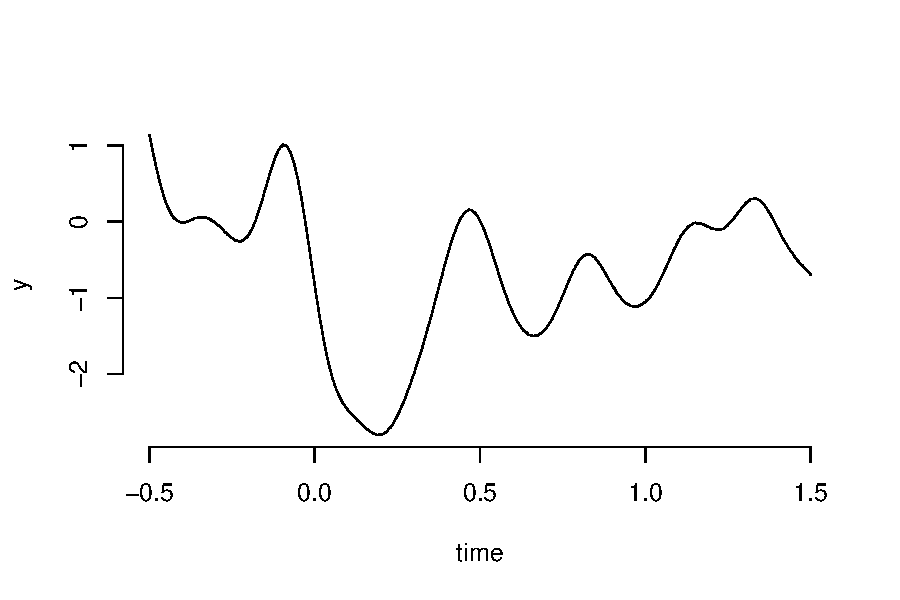
\includegraphics[width=\maxwidth]{figure/unnamed-chunk-4-1} 

}



\end{knitrout}

Now we have computed a realisation $f(t)$ of a GP with excellent sampling and precision, we now make it more like real data by keeping only a few samples and adding random noise to each value.

\begin{equation}
  y(t_i) = f(t_i) + \epsilon_i
\end{equation}

where $t_i$ are a few randomly chosen times, and $\epsilon_i$ are independently distributed random variates with standard deviation $\sigma_i$: $\epsilon \sim N(0, \sigma_i)$.

\begin{knitrout}
\definecolor{shadecolor}{rgb}{0.969, 0.969, 0.969}\color{fgcolor}\begin{kframe}
\begin{alltt}
\hlcom{# now observe f(t) only at n random times}
\hlstd{n} \hlkwb{<-} \hlnum{35}
\hlstd{indx} \hlkwb{<-} \hlkwd{sample}\hlstd{(}\hlnum{126}\hlopt{:}\hlnum{375}\hlstd{,} \hlkwc{size} \hlstd{= n)}
\hlstd{indx} \hlkwb{<-} \hlkwd{sort}\hlstd{(indx)}
\hlstd{t} \hlkwb{<-} \hlstd{t.f[indx]}
\hlstd{y} \hlkwb{<-} \hlstd{f[indx]}

\hlcom{# now add measurement errors}
\hlstd{dy} \hlkwb{<-} \hlkwd{rep}\hlstd{(}\hlnum{0.1}\hlstd{, n)}
\hlstd{epsilon} \hlkwb{<-} \hlkwd{rnorm}\hlstd{(n,} \hlkwc{mean} \hlstd{=} \hlnum{0}\hlstd{,} \hlkwc{sd} \hlstd{= dy)}
\hlstd{y} \hlkwb{<-} \hlstd{y} \hlopt{+} \hlstd{epsilon}

\hlcom{# plot the observations}
\hlkwd{points}\hlstd{(t, y,} \hlkwc{pch} \hlstd{=} \hlnum{1}\hlstd{)}

\hlcom{# plot error bars}
\hlkwd{segments}\hlstd{(t, y}\hlopt{-}\hlstd{dy, t, y}\hlopt{+}\hlstd{dy)}
\end{alltt}
\end{kframe}

{\centering 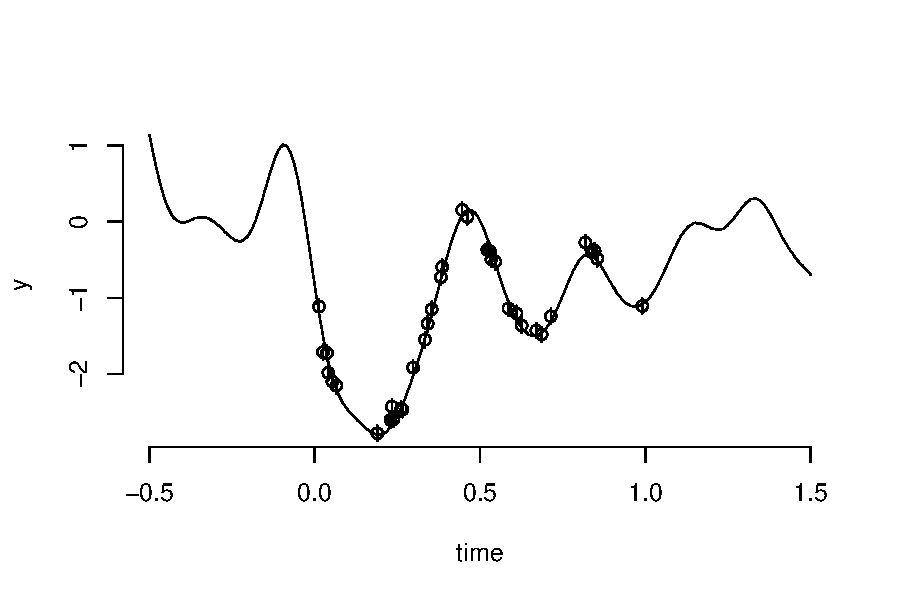
\includegraphics[width=\maxwidth]{figure/unnamed-chunk-5-1} 

}



\end{knitrout}

Now let's \emph{reconstruct} $y(t)$ based on just the `observed' (i.e. noisy) data points.

\begin{knitrout}
\definecolor{shadecolor}{rgb}{0.969, 0.969, 0.969}\color{fgcolor}\begin{kframe}
\begin{alltt}
\hlcom{# times for reconstruction}
  \hlstd{m} \hlkwb{<-} \hlnum{120}
  \hlstd{t.star} \hlkwb{<-} \hlkwd{seq}\hlstd{(}\hlopt{-}\hlnum{0.5}\hlstd{,} \hlnum{1.5}\hlstd{,} \hlkwc{length} \hlstd{= m)}

\hlcom{# compute model covariance matrix at observed delays}
  \hlstd{tau.obs} \hlkwb{<-} \hlkwd{abs}\hlstd{(} \hlkwd{outer}\hlstd{(t, t,} \hlstr{"-"}\hlstd{) )}
  \hlstd{K} \hlkwb{<-} \hlkwd{acv}\hlstd{(tau.obs, theta)}

\hlcom{# compute matrix of covariances between observations and predictions}
  \hlstd{tau.ki} \hlkwb{<-} \hlkwd{abs}\hlstd{(} \hlkwd{outer}\hlstd{(t.star, t,} \hlstr{"-"}\hlstd{) )}
  \hlstd{tau.kk} \hlkwb{<-} \hlkwd{abs}\hlstd{(} \hlkwd{outer}\hlstd{(t.star, t.star,} \hlstr{"-"}\hlstd{) )}
  \hlstd{K.ki} \hlkwb{<-} \hlkwd{acv}\hlstd{(tau.ki, theta)}
  \hlstd{K.ik} \hlkwb{<-} \hlkwd{t}\hlstd{(K.ki)}
  \hlstd{K.kk} \hlkwb{<-} \hlkwd{acv}\hlstd{(tau.kk, theta)}
  \hlkwd{rm}\hlstd{(tau.obs, tau.ki, tau.kk)}
\end{alltt}
\end{kframe}
\end{knitrout}

We used the {\tt rm()} function to delete from memory the arrays that we no longer need. (Otherwise we have lots of large arrays left over from the calculation.)

Now let's check everything has the right shape. Here {\tt K} is the matrix $K(t, t)$ [$n \times n$] containing the ACV values between all the observation times, $t$. {\tt K.ki} is the matrix $K(t_*, t)$ [$m \times n$] containing the ACV values between the $m$ prediction times, $t_*$, and the $n$ observation times, $t$. {\tt K.ik} is the transpose of this. {\tt K.kk} is the matrix $K(t_*, t_*)$ [$m \times m$] containing the ACV values between all the prediction times, $t_*$.

\begin{knitrout}
\definecolor{shadecolor}{rgb}{0.969, 0.969, 0.969}\color{fgcolor}\begin{kframe}
\begin{alltt}
\hlcom{# check the sizes of the matrices we have made}
  \hlkwd{dim}\hlstd{(K)}
\end{alltt}
\begin{verbatim}
## [1] 35 35
\end{verbatim}
\begin{alltt}
  \hlkwd{dim}\hlstd{(K.ki)}
\end{alltt}
\begin{verbatim}
## [1] 120  35
\end{verbatim}
\begin{alltt}
  \hlkwd{dim}\hlstd{(K.ik)}
\end{alltt}
\begin{verbatim}
## [1]  35 120
\end{verbatim}
\begin{alltt}
  \hlkwd{dim}\hlstd{(K.kk)}
\end{alltt}
\begin{verbatim}
## [1] 120 120
\end{verbatim}
\begin{alltt}
  \hlkwd{length}\hlstd{(y)}
\end{alltt}
\begin{verbatim}
## [1] 35
\end{verbatim}
\begin{alltt}
  \hlkwd{length}\hlstd{(dy)}
\end{alltt}
\begin{verbatim}
## [1] 35
\end{verbatim}
\end{kframe}
\end{knitrout}

Now we have all the matricies and vectors defined we can do the algebra. 

\begin{knitrout}
\definecolor{shadecolor}{rgb}{0.969, 0.969, 0.969}\color{fgcolor}\begin{kframe}
\begin{alltt}
\hlcom{# eqn 2.20 of R&W - add the "error" term to the covariance matrix}
  \hlstd{C} \hlkwb{<-} \hlstd{K} \hlopt{+} \hlstd{dy}\hlopt{^}\hlnum{2} \hlopt{*} \hlkwd{diag}\hlstd{(}\hlnum{1}\hlstd{,} \hlkwd{NCOL}\hlstd{(K))}

\hlcom{# compute the inverse covariance matrix}
\hlcom{# using chol() then chol2inv() is faster than using solve()}
  \hlstd{C.inv} \hlkwb{<-} \hlkwd{chol2inv}\hlstd{(} \hlkwd{chol}\hlstd{(C) )}

\hlcom{# eqn 2.23 of R&W - predict the mean value at prediction times }
  \hlstd{y.star} \hlkwb{<-} \hlkwd{as.vector}\hlstd{(K.ki} \hlopt \hlstd{C.inv} \hlopt \hlstd{y)}

\hlcom{# eqn 2.24 of R&W - predict the covariances at all prediction times}
  \hlstd{cov.star} \hlkwb{<-} \hlstd{K.kk} \hlopt{-} \hlstd{K.ki} \hlopt \hlstd{C.inv} \hlopt \hlstd{K.ik}

\hlcom{# extract the diagonal elements from the covariance}
\hlcom{# matrix, i.e. the variances at times t.pr. Store this as a vector.}
\hlcom{# Use the absolute value to avoid any negative values creeping in }
\hlcom{# due to numerical errors. Take sqrt to get standard deviation (=sigma)}
  \hlstd{dy.star} \hlkwb{<-} \hlkwd{as.vector}\hlstd{(} \hlkwd{sqrt}\hlstd{(} \hlkwd{abs}\hlstd{(} \hlkwd{diag}\hlstd{(cov.star) ) ) )}

  \hlcom{# define the output product}
  \hlstd{result} \hlkwb{<-} \hlkwd{list}\hlstd{(}\hlkwc{t} \hlstd{= t.star,} \hlkwc{y} \hlstd{= y.star,} \hlkwc{dy} \hlstd{= dy.star,} \hlkwc{var} \hlstd{= cov.star)}
\end{alltt}
\end{kframe}
\end{knitrout}

I suspect it is possible to make the above lines of matrix algebra faster, e.g. by avoiding explictly computing the $[n \times n]$ matrix inverse $C^{-1}$, and by not repeating the $K(t_*, t) C^{-1}$ matrix multiplication $[m \times n] \times [n \times n]$.

Now plot the results.

\begin{knitrout}
\definecolor{shadecolor}{rgb}{0.969, 0.969, 0.969}\color{fgcolor}\begin{kframe}
\begin{alltt}
\hlcom{# plot the reconstruction mean}
  \hlkwd{lines}\hlstd{(result}\hlopt{$}\hlstd{t, result}\hlopt{$}\hlstd{y,} \hlkwc{col} \hlstd{=} \hlstr{"blue"}\hlstd{,} \hlkwc{lwd} \hlstd{=} \hlnum{3}\hlstd{)}

\hlcom{# plot a 'snake' of the mean +/-2 standard deviations}
  \hlkwd{lines}\hlstd{(result}\hlopt{$}\hlstd{t, result}\hlopt{$}\hlstd{y}\hlopt{-}\hlnum{2}\hlopt{*}\hlstd{result}\hlopt{$}\hlstd{dy,} \hlkwc{col} \hlstd{=} \hlstr{"blue"}\hlstd{,} \hlkwc{lwd} \hlstd{=} \hlnum{1}\hlstd{)}
  \hlkwd{lines}\hlstd{(result}\hlopt{$}\hlstd{t, result}\hlopt{$}\hlstd{y}\hlopt{+}\hlnum{2}\hlopt{*}\hlstd{result}\hlopt{$}\hlstd{dy,} \hlkwc{col} \hlstd{=} \hlstr{"blue"}\hlstd{,} \hlkwc{lwd} \hlstd{=} \hlnum{1}\hlstd{)}
\end{alltt}
\end{kframe}

{\centering 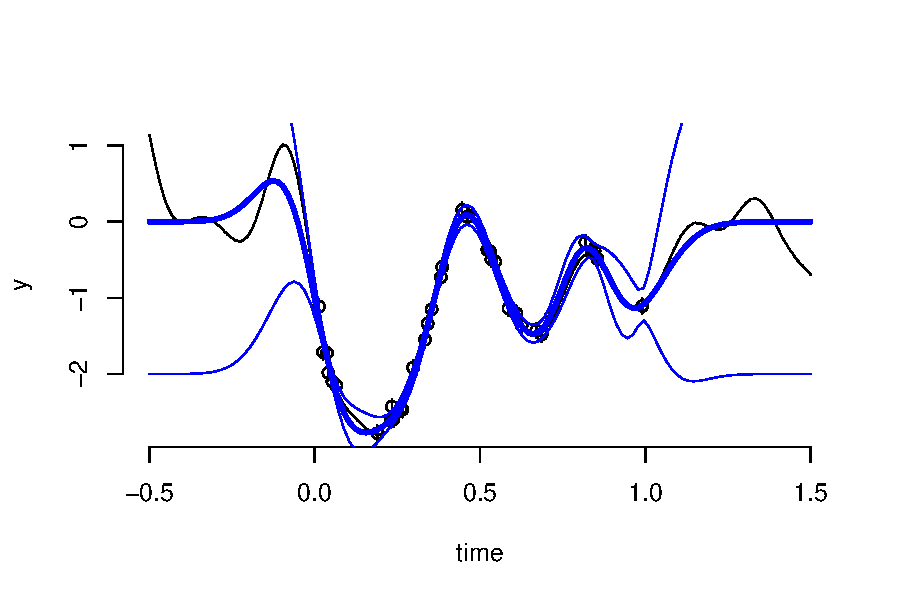
\includegraphics[width=\maxwidth]{figure/unnamed-chunk-9-1} 

}



\end{knitrout}

%%%%%%%%%%%%%%%%%%%%%%%%%%%%%%%%%%%%%%%%%%%%%%%
\vspace{0.4cm}
\textbf{Reconstructing a Gaussian Process}
\\

Why is this useful? It means that if we know some values of $\mathbf{y}$ we can make a more informed estimate of what the other values of $\mathbf{y}$ are. If we know $\mathbf{y}_2$ we can write down or compute using the conditional distribution of $\mathbf{y}_2$. In practice, this means that if we are studying some random Gaussian process, and we have a few observations at times $\mathbf{t_2}$ we can write down the distribution of un-observed values for any other times $\mathbf{t_1}$.

This is often useful for interpolation (estimate values of $y$ between two observations), or extrapolation to times before/after all available observations (e.g. forecasting future values). I call these together \emph{reconstruction}. We can start with a noisy and irregularly spaced series of observations, plus knowledge of the covariance structure of the process that produced the observations, and compute the full conditional distribution (Gaussian mean and covariance) for the process at any set of times.

There is a very detailed discussion of using GP theory for reconstruction in G. B. Rybicki \& W. H. Press (1992; Astrophysical Journal, v389, pp169-176). 

But, the above assumes we know $ACV(\tau)$ and can therefore compute $\Sigma$ for any (observed or prediction) times. How do we know what this function should be? And how to we know $\bmu =0$? We will address these points later.

\end{document}
